\documentclass[12pt,a4paper]{article}
\usepackage{fontspec}\usepackage{polyglossia}\setdefaultlanguage{ukrainian}
\setmainfont{NewComputerModern10}\setsansfont{Noto Sans}\setmonofont{Noto Sans Mono}[Scale=0.82]
\usepackage{amsmath,amssymb,booktabs,caption,enumitem,float,geometry,graphicx,hyperref,microtype,titlesec,xcolor}
\geometry{left=2cm,right=2cm,top=2cm,bottom=2cm}\setlength{\parindent}{1.25cm}\linespread{1.08}
\titleformat{\section}{\normalfont\fontsize{14}{16}\selectfont\bfseries}{\thesection}{0.6em}{}
\titlespacing*{\section}{0pt}{1.4em}{0.65em}\captionsetup{font=small,labelfont=bf,labelsep=endash}
\usepackage[newfloat]{minted}\SetupFloatingEnvironment{listing}{name=Лістинг}
\setminted{fontsize=\footnotesize,linenos,breaklines,autogobble,frame=single,framesep=2mm,bgcolor=gray!5,tabsize=4}
\hypersetup{unicode,colorlinks=true,linkcolor=black,pdftitle={ІО-41, Давидчук А. М., Лабораторна робота №3},pdfauthor={Давидчук Артем}}
\newcommand{\resultDir}{../results}\newcommand{\studentGroup}{ІО-41}\newcommand{\studentName}{Давидчук А. М.}\newcommand{\reportYear}{2026}
\begin{document}\pagenumbering{gobble}
\begin{titlepage}\begin{center}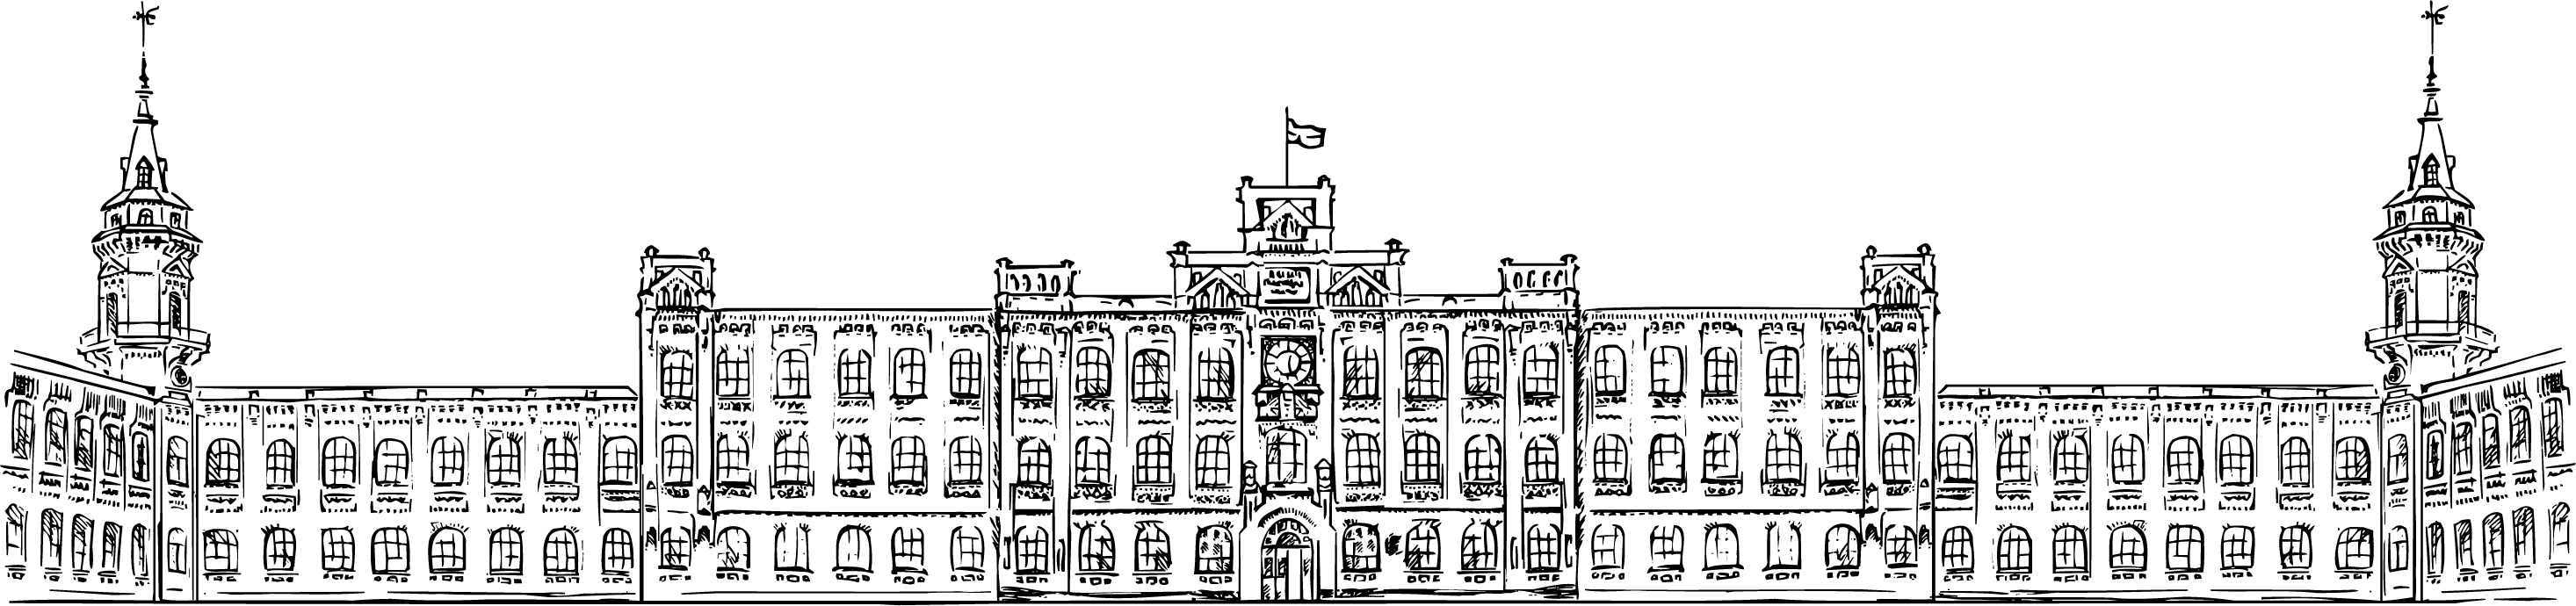
\includegraphics[width=.7\textwidth]{../../../../../../templates/letterhead.png}\end{center}
\begin{center}\large Національний технічний університет України\\ «Київський політехнічний інститут імені Ігоря Сікорського»\\[1em]Факультет інформатики та обчислювальної техніки\\Кафедра обчислювальної техніки\end{center}\vfill
\begin{center}\textbf{\LARGE Методи та технології штучного інтелекту}\\[2em]\textbf{\Large Лабораторна робота №3}\\[.7em]«Дослідження алгоритму нечіткої кластеризації»\end{center}\vfill
\begin{flushright}\begin{minipage}{.48\textwidth}Виконав: студент 3 курсу ФІОТ,\\групи \studentGroup\\\textit{\studentName}\\Перевірив: \textit{Польшакова О. М.}\end{minipage}\end{flushright}\vfill\begin{center}Київ --- \reportYear\end{center}\end{titlepage}\pagenumbering{arabic}

\section{Тема та мета роботи}
\noindent\textbf{Тема:} дослідження алгоритму нечіткої кластеризації.\\
\noindent\textbf{Мета:} розв'язати практичну задачу автоматичної класифікації об'єктів методами нечіткої логіки, знайти центри кластерів та дослідити зміну цільової функції.

\section{Постановка задачі}
Розглянуто задачу сегментації мережевих пристроїв за двома ознаками: середньою затримкою відповіді та кількістю пакетів за хвилину. Така постановка відповідає практичній задачі моніторингу мережі: пристрої з подібною поведінкою мають потрапити до однієї групи, але пристрої на межі груп не повинні примусово отримувати лише одну мітку.

Для експерименту згенеровано 360 двовимірних об'єктів, які утворюють три групи. Кожен об'єкт має вигляд $x_k=(x_{k1},x_{k2})$, де $x_{k1}$ --- затримка у мілісекундах, а $x_{k2}$ --- кількість пакетів за хвилину. Необхідно визначити три нечіткі кластери алгоритмом Fuzzy C-Means, знайти їхні центри, показати розподіл об'єктів на площині та проаналізувати збіжність.

\section{Теоретичні відомості}
Кластеризація є навчанням без учителя: на початку для об'єктів не задані правильні класи. Алгоритм сам шукає групи за відстанями між об'єктами. У жорсткій кластеризації об'єкт належить лише одному кластеру. У нечіткій кластеризації кожен об'єкт може належати всім кластерам із різними ступенями належності.

Матриця належності $U=[u_{jk}]$ містить ступінь належності об'єкта $k$ до кластера $j$. Для кожного об'єкта виконується умова $\sum_j u_{jk}=1$. Наприклад, вектор належності $(0{,}1;0{,}8;0{,}1)$ означає, що об'єкт переважно належить другому кластеру, але повністю не виключається його належність до інших груп.

Центр кластера обчислюється як зважене середнє:
\begin{equation}c_j=\frac{\sum_k u_{jk}^q x_k}{\sum_k u_{jk}^q}.\end{equation}
Показник $q$ визначає, наскільки сильно враховуються великі ступені належності. У роботі використано стандартне значення $q=2$. Цільова функція FCM:
\begin{equation}J=\sum_j\sum_k u_{jk}^q\lVert x_k-c_j\rVert^2.\end{equation}
Чим ближче об'єкт до центра, тим більшим буде його ступінь належності до відповідного кластера. Після оновлення центрів ступені належності перераховуються за відстанями до центрів. Ітерації завершуються, коли норма зміни матриці належності стає меншою за задану похибку або досягнуто максимальну кількість ітерацій. Зменшення $J$ використовується як додаткова ознака того, що алгоритм рухається до стабільного розподілу.

\section{Алгоритм і програмна реалізація}
Використано параметри: кількість кластерів $3$, показник нечіткості $q=2$, точність $0{,}005$ та максимум 100 ітерацій. Три кластери обрано відповідно до трьох синтетичних груп пристроїв. Значення $q=2$ є типовим компромісом між жорстким і дуже розмитим розподілом. Реалізація алгоритму виконана мовою Python без готового класифікатора, тому кожен етап FCM реалізовано явно.

Спочатку генерується початкова матриця належності випадковим способом і нормується по кожному об'єкту. Далі повторюються чотири дії: обчислення ваг $u_{jk}^q$, обчислення центрів, обчислення відстаней і оновлення матриці належності. Після цього перевіряється норма різниці між новою та попередньою матрицями.
\begin{listing}[H]\begin{minted}{python}
weights = membership ** fuzziness
centers = (weights @ data) / weights.sum(axis=1, keepdims=True)
distances = np.linalg.norm(data[None, :, :] - centers[:, None, :], axis=2)
ratios = (distances[:, None, :] / distances[None, :, :]) ** (2 / (fuzziness - 1))
membership = 1 / ratios.sum(axis=1)
\end{minted}
\caption{Основні операції Fuzzy C-Means}
\end{listing}

\section{Результати}
Алгоритм завершив роботу за 10 ітерацій. Отримані центри наведено в таблиці. Перший кластер відповідає пристроям із малою затримкою та невеликою кількістю пакетів. Другий кластер має найбільшу затримку й середню інтенсивність трафіку. Третій кластер характеризується великою кількістю пакетів за хвилину та середньою затримкою.
\begin{table}[H]\centering\begin{tabular}{lrr}\toprule Кластер & Затримка, мс & Пакети за хвилину\\\midrule 1&19,6275&19,7072\\2&75,9408&54,9096\\3&44,1475&109,4671\\\bottomrule\end{tabular}\caption{Центри нечітких кластерів}\end{table}
\begin{figure}[H]\centering\includegraphics[width=.83\textwidth]{\resultDir/clusters.png}\caption{Об'єкти та центри кластерів}\end{figure}
\begin{figure}[H]\centering\includegraphics[width=.78\textwidth]{\resultDir/objective.png}\caption{Зміна цільової функції FCM}\end{figure}

На графіку кластерів видно три компактні області, а чорні зірочки розташовані приблизно в центрах цих областей. Це означає, що за вибраними ознаками синтетичні групи добре відокремлюються. На графіку цільової функції спостерігається швидке зменшення на перших ітераціях і майже горизонтальна ділянка після восьмої ітерації. Отже, подальші ітерації вже майже не змінюють результат.

Матриця належності та числові центри додатково збережені у файлах \texttt{membership\_matrix.csv} і \texttt{cluster\_centers.csv}. Це дає змогу перевірити не лише остаточну мітку, а й ступінь упевненості алгоритму для кожного об'єкта.

\section{Висновки}
Побудовано систему нечіткої кластеризації мережевих пристроїв за двома ознаками. FCM розділив 360 об'єктів на три кластери та знайшов їхні центри. Зменшення цільової функції на ітераціях підтверджує збіжність алгоритму. На відміну від жорсткої кластеризації, FCM зберігає ступені належності об'єктів до всіх кластерів, тому краще описує об'єкти на межах груп.

\section{Контрольні питання}
\begin{enumerate}[leftmargin=*]
\item \textit{Що таке кластеризація і яке її основне призначення?}\\
Кластеризація --- це поділ об'єктів на групи за схожістю без наперед заданих правильних міток. Її призначення --- виявити структуру даних.
\item \textit{У чому відмінність кластеризації від класифікації?}\\
Класифікація навчається на відомих класах, а кластеризація самостійно шукає групи у невідомих даних.
\item \textit{Які основні підходи до кластеризації існують?}\\
Ієрархічний, центроїдний, щільнісний, модельний та нечіткий підходи.
\item \textit{Що таке жорстка кластеризація?}\\
Це кластеризація, у якій кожен об'єкт отримує рівно одну мітку кластера.
\item \textit{Які недоліки має жорстка кластеризація?}\\
Вона різко розділяє простір і не показує невизначеність об'єктів, що лежать між групами.
\item \textit{У чому полягає суть нечіткої кластеризації?}\\
Кожен об'єкт отримує ступінь належності до кожного кластера, а не лише одну мітку.
\item \textit{Що таке матриця приналежності?}\\
Це матриця, рядки якої відповідають кластерам, а стовпці --- об'єктам; її елементи є ступенями належності.
\item \textit{Які основні етапи алгоритму FCM?}\\
Ініціалізація матриці, обчислення центрів, оновлення належностей і перевірка умови зупинки.
\item \textit{Чим відрізняються K-means та Fuzzy C-Means?}\\
K-means формує жорсткі кластери, а FCM зберігає часткову належність об'єктів до всіх кластерів.
\item \textit{Як інтерпретується ступінь належності 0,8?}\\
Це означає сильну належність об'єкта до кластера, але не абсолютну гарантію належності.
\item \textit{Які переваги нечіткої кластеризації?}\\
Вона краще працює з перехідними областями, шумом і об'єктами, які мають ознаки кількох груп.
\item \textit{Де застосовується нечітка кластеризація?}\\
У медицині, сегментації зображень, маркетингу, аналізі поведінки користувачів і мережевому моніторингу.
\item \textit{Які обмеження FCM?}\\
Результат залежить від початкової матриці, масштабу ознак, кількості кластерів і показника нечіткості.
\item \textit{Як підвищити якість кластеризації?}\\
Можна нормувати ознаки, запускати алгоритм із різними ініціалізаціями та підбирати кількість кластерів.
\item \textit{Як FCM поєднують з іншими методами?}\\
Результати FCM можна подавати на вхід класифікатору, нейромережі або використовувати разом із PCA для зменшення розмірності.
\end{enumerate}
\end{document}
